\documentclass[a4paper,11pt]{report}
%\documentclass{foils}

\usepackage{geometry,graphicx}
\usepackage{verbatim}
\usepackage{url}
\usepackage{fancybox}
\usepackage{fancyhdr}
\usepackage{framed}
\usepackage{color}
\usepackage{multirow}

\usepackage{lingmacros}  % included with GenI
\usepackage{covington}   % included with GenI

% ----------------------------------------
\newcommand{\jargon}{\textbf}
\newcommand{\natlang}{\textit}
\newcommand{\semexpr}{\texttt}
\newcommand{\tautree}[1] {$\tau_{#1}$}
\newcommand{\koweytree}{\texttt}
\long\def\ignore#1{}

\newcommand{\fnparam}{\texttt}
\newcommand{\fnref}[1]{\textit{#1} (page \pageref{fn:#1})}
\newcommand{\fnreflite}[1]{\textit{#1}}
\newcommand{\fnlabel}[1]{\paragraph{#1}\label{fn:#1}}

\newcommand{\tuple}[1]{\langle #1 \rangle}
\setcounter{chapter}{-1}
\setcounter{secnumdepth}{3}
% ----------------------------------------

\geometry{verbose,tmargin=40mm,bmargin=40mm,lmargin=25mm,rmargin=25mm}
%\input{lambdaTeX}

\pagestyle{fancyplain} 
\lfoot{GenI source code}
\cfoot{\thepage}
\rfoot{}

%\setlength\parindent{0pt}
\setlength{\fboxsep}{0.1pt}

\renewcommand\FrameHeightAdjust{1pt}


\newenvironment{framedcode}% using default \FrameCommand
  {\MakeFramed {\advance\hsize-\width \FrameRestore}}%
  {\endMakeFramed}

\newenvironment{includecodeinmanual}
  {}
  {}

\newenvironment{code}% using default \FrameCommand
  {\VerbatimEnvironment
   \footnotesize
   %\begin{framedcode}
   \begin{Verbatim}
  }%
  {\end{Verbatim} 
   %\end{framedcode}
   \normalsize }

%\lstloadlanguages{Haskell} 
%\lstnewenvironment{code} 
%    {\lstset{}% 
%      \csname lst@SetFirstLabel\endcsname} 
%    {\csname lst@SaveFirstLabel\endcsname} 
%    \lstset{ 
%      basicstyle=\small\ttfamily, 
%      flexiblecolumns=false, 
%      basewidth={0.5em,0.45em}, 
%      literate={-}{{$-$}}1 {+}{{$+$}}1 {/}{{$/$}}1 {*}{{$*$}}1 {=}{{$=$}}1 
%               {>}{{$>$}}1 {<}{{$<$}}1 {\\}{{$\lambda$}}1 
%               {->}{{$\rightarrow$}}2 {>=}{{$\geq$}}2 {<-}{{$\leftarrow$}}2 
%               {<=}{{$\leq$}}2 {=>}{{$\Rightarrow$}}2 {\ .}{{$\circ$}}2 
%               {>>}{{>>}}2 {>>=}{{>>=}}2 
%    } 

\begin{document}
\title{Literate GenI}
\author{TALARIS\\LORIA}

\maketitle
\tableofcontents

% -------------------------------------------------------------------------
% Overview 
% -------------------------------------------------------------------------

\chapter*{License}

GenI surface realiser\\
Copyright \copyright 2005-2007 Carlos Areces and Eric Kow

\bigskip

This program is free software; you can redistribute it and/or
modify it under the terms of the GNU General Public License
as published by the Free Software Foundation; either version 2
of the License, or (at your option) any later version.

\bigskip

This program is distributed in the hope that it will be useful,
but WITHOUT ANY WARRANTY; without even the implied warranty of
MERCHANTABILITY or FITNESS FOR A PARTICULAR PURPOSE.  See the
GNU General Public License for more details.

\bigskip

You should have received a copy of the GNU General Public License
along with this program; if not, write to the Free Software
Foundation, Inc., 59 Temple Place - Suite 330, Boston, MA  02111-1307, USA.

\chapter{Overview}

\begin{figure}[h]
\begin{center}
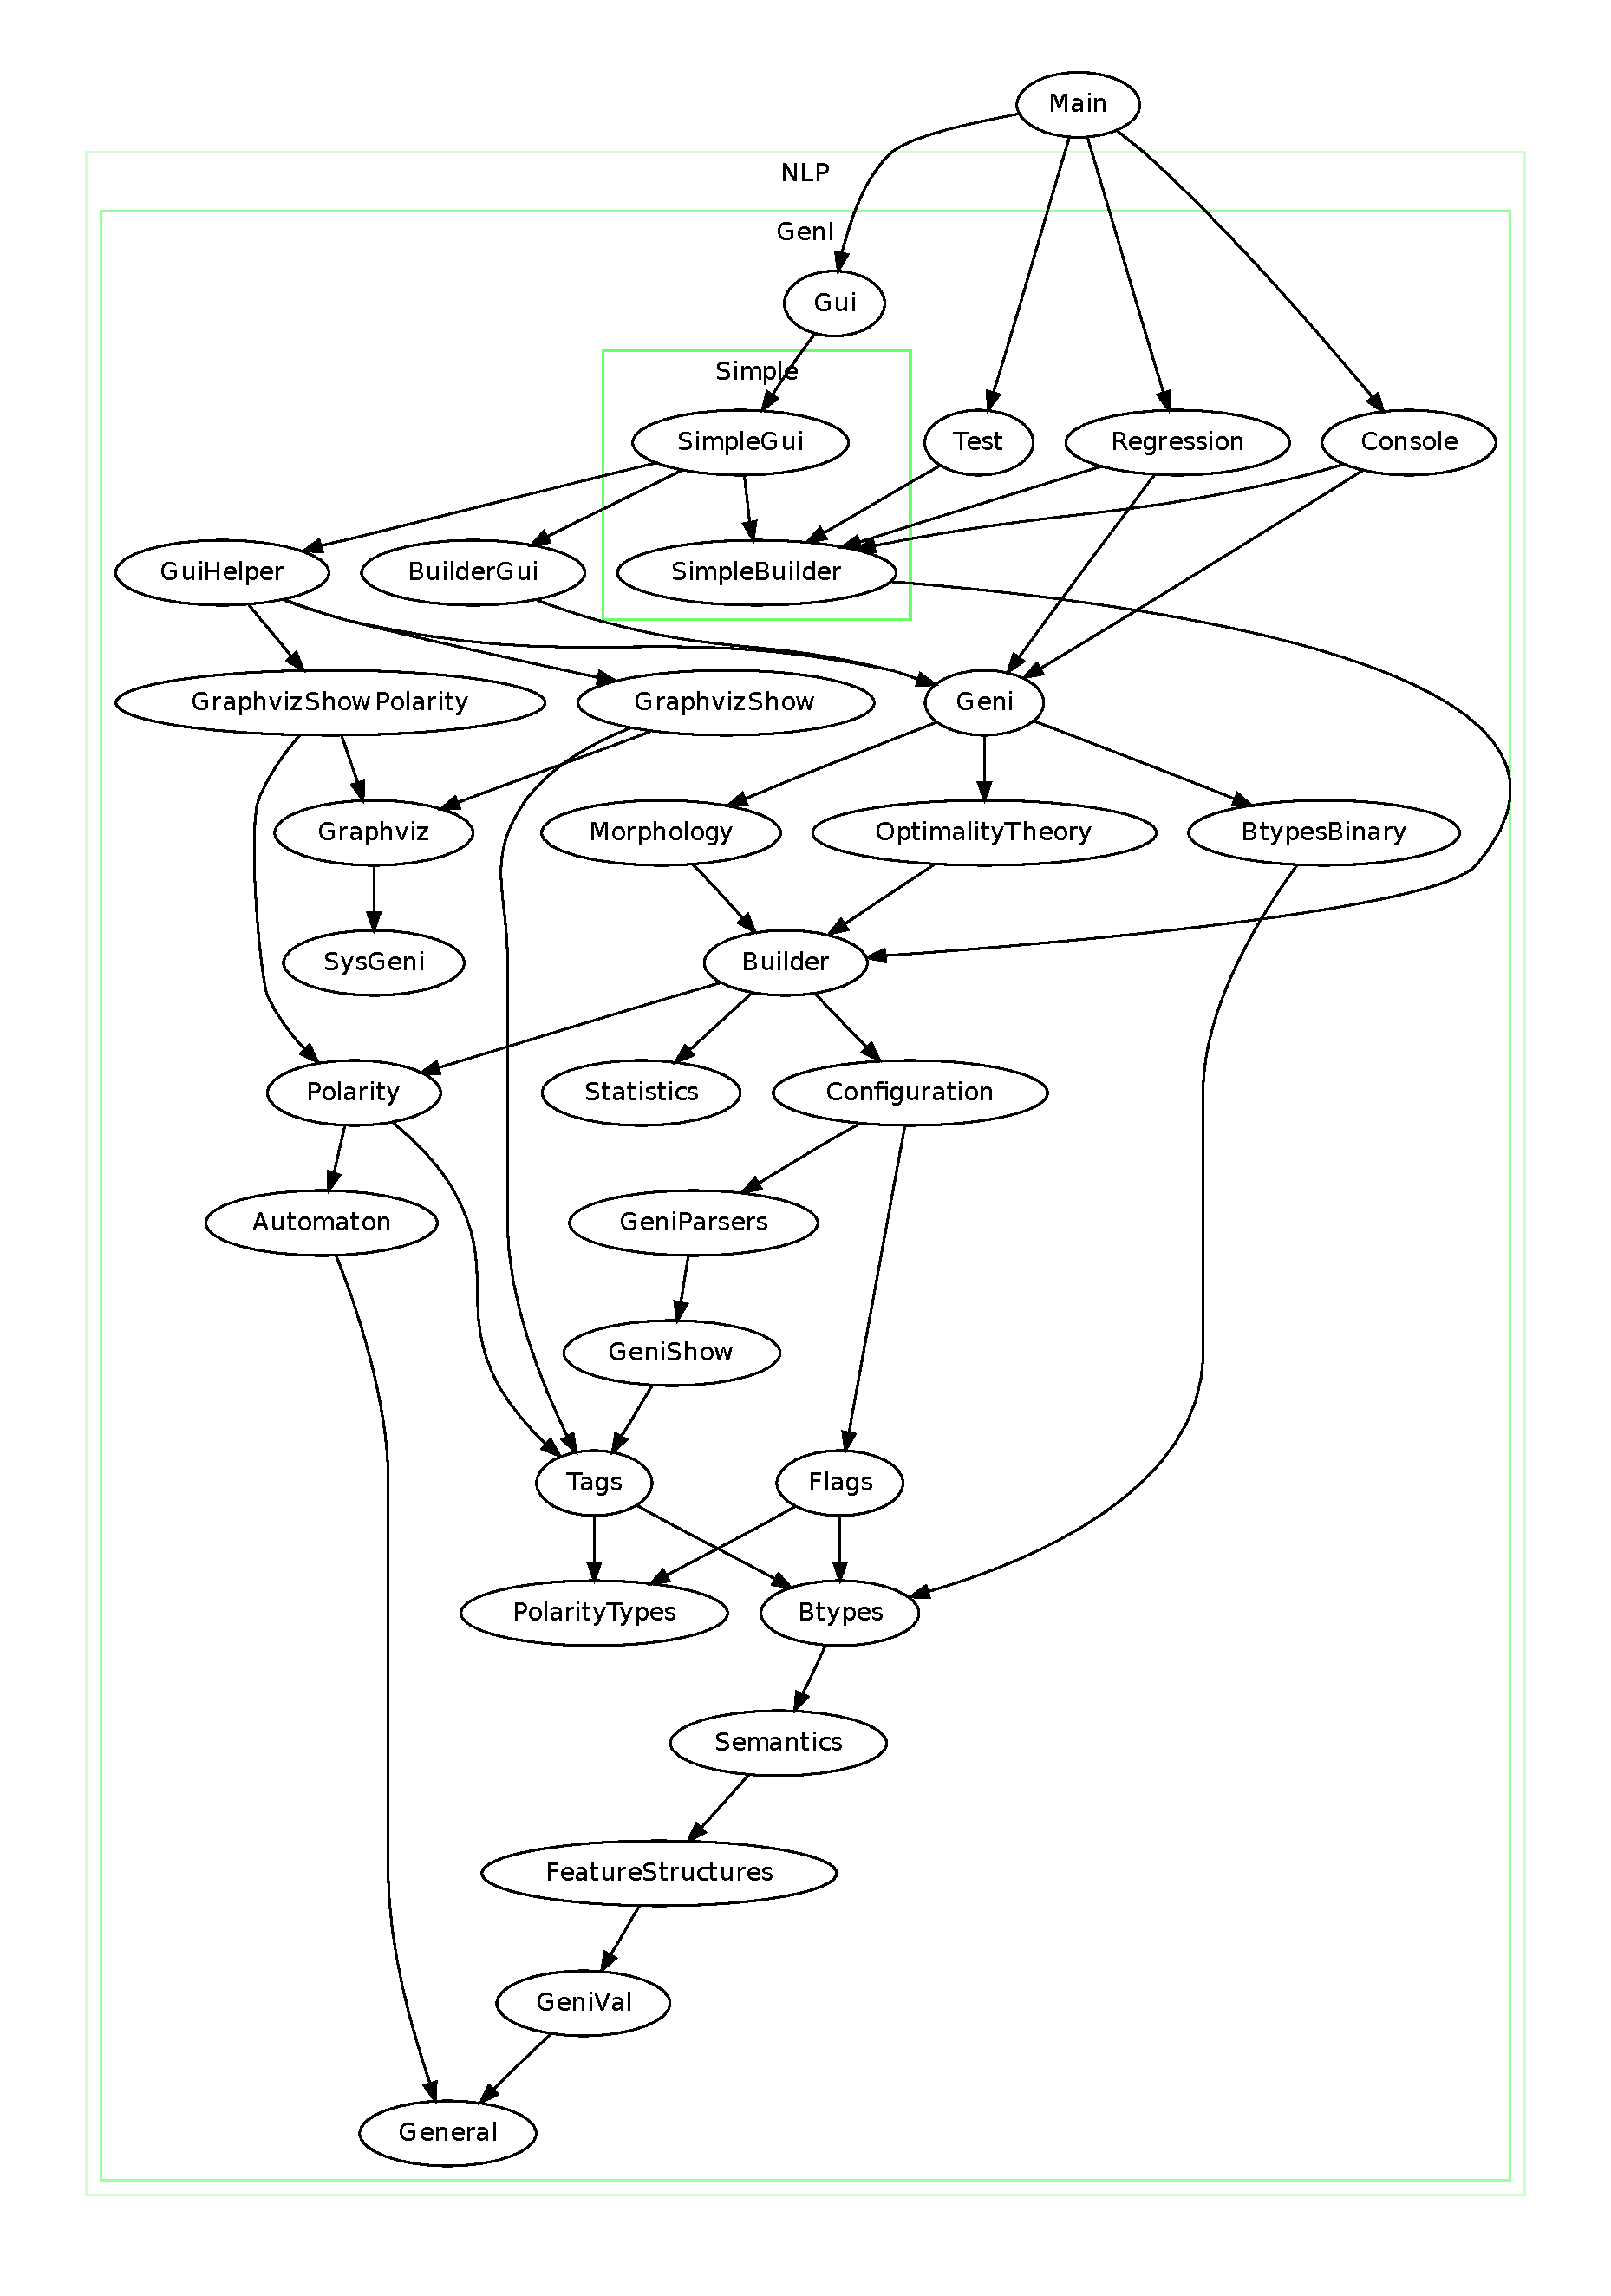
\includegraphics[scale=0.5]{images/genidep}
\caption{Transitive reduction of module dependencies}
\end{center}
\end{figure}

This document contains the source code to the GenI generator 
partly adapted to a literate programming style.  

\section{Core files and Builders}

The modules where the most action happens are GenI (chapter
\ref{cha:geni}) which acts as an interface between the front end and
backend(s) and also takes care of lexical selection.

Otherwise, you probably want to look at the various Builders in
\ref{prt:builders}.  This is where all the chart generation stuff
happens.

The other core modules provide basic data structures and operations
like feature structure unification.

\section{Enhancements}

This portion is for optimisations and other optional features of the
generator.
In addition to the modules below, chapter \ref{chp:other_optimisations}
will point you to ones which could not be cleanly seperated into
modules.

\begin{description}
 \item[Morphology.lhs]
 \item[Polarity.lhs]   - the polarity automaton optimisation 
\end{description}

\section{Miscellaneous}

For reference, we also include in chapter \label{cha:GeniParsers} the
parsers for all GenI formats (macros, lexicon, input semantics).  These
are all written in Parsec.  They used to be written in Happy, but I
eventually found that hard to maintain and extend.

There are also many modules which I have removed from this document,
mostly the user interface code.  See chapter \ref{cha:other} for
details.  One idea which might be interesting is to make the user
interface documentation just be the users manual, \`a la darcs.

% -------------------------------------------------------------------------
% future literate notes
% -------------------------------------------------------------------------

\input{../src/MainGeni.lhs}

\part{Core files}

\input{../src/NLP/GenI/Geni.lhs}
\input{../src/NLP/GenI/Btypes.lhs}
\input{../src/NLP/GenI/Tags.lhs}

\part{Builders}
\label{prt:builders}

\input{../src/NLP/GenI/Builder.lhs}
\input{../src/NLP/GenI/Simple/SimpleBuilder.lhs}
\input{../src/NLP/GenI/CkyEarley/CkyBuilder.lhs}

\part{Optional}

\input{../src/NLP/GenI/Morphology.lhs}
\input{../src/NLP/GenI/Polarity.lhs}

\chapter{Other optimisations}
\label{chp:other_optimisations}

Some of the optimisations related to adjunction are integrated into
to the generator.

\section{Semantic filtering}

See section \ref{sec:semfilter}

\section{Ordered adjunction}

See section \ref{sec:ordered_adjunction}

\section{Foot constraint}

See section \ref{sec:foot_constraint}

\part{Miscellaneous}

\input{../src/NLP/GenI/GeniParsers.lhs}
%\input{GrammarXml.lhs}
%\input{Converter.lhs}

\chapter{Other source code}
\label{cha:other}

Some parts of the GenI source code do not appear to be adapted to the
literate programming style: they are not included in this document.

\section{User interface}

\begin{enumerate}
\item{Console.hs}
\item{Gui.lhs}
\item{GuiHelper.lhs}
\item{Simple/SimpleGui.lhs}
\item{Cky/CkyGui.lhs}
\item{Graphviz.hs}
\end{enumerate}

\section{Bits and pieces}

\begin{enumerate}
\item{Configuration.lhs}
\item{General.hs}
\item{SysGeni.hs}
\end{enumerate}

{
\bibliographystyle{alpha}
\bibliography{genidoc}
}

\end{document}
